\begin{section}{Ejercicio 7}
Realizar un gráfico de los ECM con $b = 1$ y $n =$ 15, 30, 50, 100, 150, 200 ¿Que observa? ¿Que
estimador elige? ¿Que sospecha sobre la consistencia de los estimadores?

\begin{subsection}{Implementación}~\\
Se utiliza el siguiente código para generar los vectores.
\begin{verbatim}
b = 1;
ni = double();
ni <- c(15, 30, 50, 100, 150, 200);
niLen = 6;
momSims = double();
medSims = double();
mvSims = double();

for(i in 1:niLen){
	momSims[i] <- simulacion_mom(b,ni[i]);
	medSims[i] <- simulacion_med(b,ni[i]);
	mvSims[i] <- simulacion_mv(b,ni[i]);
}

\end{verbatim}

se crean luego los gráficos compuestos con el siguiente código:

\begin{verbatim}

> plot(ni, momSims, ylim=c(0,0.030))
> points(ni, medSims , col="red")
> points(ni, mvSims , col="green")
> 
\end{verbatim}


\end{subsection}
\newpage
\begin{subsection}{Resultados}~\\

Se obtiene el siguiente gráfico, donde los puntos de color negro son los de $B_{mom}$, los de color rojo los de $B_{med}$, y los de color verde los de $B_{mv}$.\\


Error cuadratico medio de $B_{mom}$
\begin{figure}[H]
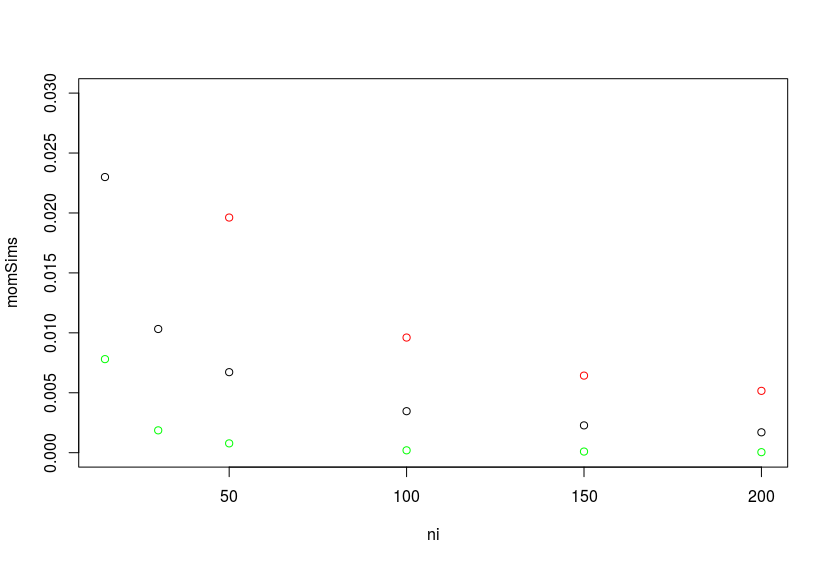
\includegraphics[scale=0.65]{plots/combNPlot.png}
\centering
\end{figure}
~\\
~\\
Nuevamente se observa una convergencia mas rápida para el estimador de máxima verosimilitud. Ademas, en cuanto a la consistencia, el único estimador que converge al valor real, al menos con $n<200$, es el de máxima verosimilitud, con lo cual es el único que parece consistente.
\end{subsection}
\end{section}